\documentclass[letterpaper,10pt,titlepage]{article}

\usepackage{graphicx}                                        
\usepackage{amssymb}                                         
\usepackage{amsmath}                                         
\usepackage{amsthm}                                          

\usepackage{alltt}                                           
\usepackage{float}
\usepackage{color}
\usepackage{url}

%\usepackage{balance}
%\usepackage[TABBOTCAP, tight]{subfigure}
%\usepackage{enumitem}
\usepackage{pstricks, pst-node}

\usepackage{geometry}
\geometry{textheight=9in, textwidth=6.5in}

%random comment

\newcommand{\cred}[1]{{\color{red}#1}}
\newcommand{\cblue}[1]{{\color{blue}#1}}

\usepackage{hyperref}
\usepackage{geometry}

\def\name{Jacob Branaugh, Brenn Kucey}

%% The following metadata will show up in the PDF properties
\hypersetup{
  colorlinks = true,
  urlcolor = black,
  pdfauthor = {\name},
  pdfkeywords = {cs472 ``computer architecture'' clements ``chapter 2''},
  pdftitle = {CS 472: Homework 2},
  pdfsubject = {CS 472: Homework 2},
  pdfpagemode = UseNone
}

\begin{document}
\hfill \name

\hfill \today

\hfill CS 472 HW 2

\begin{enumerate}
\item[(2.5)] Calculations are to be performed to a precision of 0.001\%. How many bits
	does this require?
  \item[\textbullet] This precision requires 10 bits. 0.001 can be represented as
	$\frac{1}{1000}$. $2^{-9}$ is equal to $\frac{1}{512}$ and $2^{-10}$ is equal to
	$\frac{1}{1024}$. Since $\frac{1}{1000}$ is less than $\frac{1}{512}$, 9 bits is
	too few. However, since $\frac{1}{1000}$ is greater than $\frac{1}{1024}$, 10
	bits is sufficient.

\item[(2.13)] Perform the following calculations in the stated bases:
  \\
  \\
  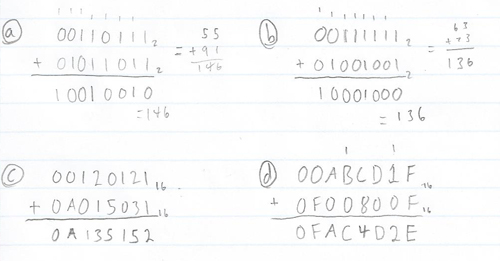
\includegraphics{problem13.jpg}

\item[(2.14)] What is arithmetic overflow? When does it occur and how can it be detected?
  \item[\textbullet] Arithmetic overflow is when the number of bits necessary to represent
	  a binary number exceed the number of bits available to represent the number.
	  It can be detected by the overflow flag of the status register being set.

\item[(2.16)] Convert 1234.125 into 32-bit IEEE floating-point format.
  \item[\textbullet] The following
    \begin{enumerate} 
      \item[-] Whole number = 1234, decimal = .125
      \item[-] $1234_{10} = 10011010010_{2}$
      \item[-] $.125_{10} = .001_{2}$
      \item[-] Mantissa = 00100...0
      \item[-] Exponent = $10_{10} + 127_{10}$ (bias) = $137_{10} = 10001001_{2}$
      \item[-] Sign = 0 (positive)
      \item[-] Floating point format =
	      {\large\textit{\textbf{0 10001001 00110100100010...0}}}
    \end{enumerate}

\item[(2.17)] What is the decimal equivalent of the 32-bit IEEE floating point value
	CC4C0000?
  \item[\textbullet] The following are the components of this floating point value:
  \begin{enumerate}
    \item[-] Sign = 1 (negative)
    \item[-] Exponent = 10011000 = 152 - 127 = {\large\textit{\textbf{25}}}
    \item[-] Significand = 1001100...0 = $\frac{1}{2}$ + $\frac{1}{16}$ + $\frac{1}{32}$ =
	    $\frac{19}{32}$ = {\large\textit{\textbf{0.59375}}}
    \item[-] Decimal number = $-1.59375 \times 2^{25}$ =
	    {\large\textit{\textbf{-53477376}}} 
  \end{enumerate}

\item[(2.22)] What is the difference between a \textit{truncation} error and a
	\textit{rounding} error?
  \item[\textbullet] A truncation error is when bits are cut off of the end (which always
	results in a round-down). A rounding error is when a number is either rounded up
	or down based on whether the unwanted bits are greater than/equal to .5 or less
	than .5, respectively. Both errors happen due to significant figure requirements.

\item[2.40] Draw a truth table for the circuit below and explain what it does:
  \item[\textbullet] This circuit is logically equivalent to an XOR. \\
    \\
    \begin{tabular}{ c c | c }
	    A & B & C \\
	    \hline
	    0 & 0 & 0 \\
	    0 & 1 & 1 \\
	    1 & 0 & 1 \\
	    1 & 1 & 0 \\
    \end{tabular}

\item[2.45] It is possible to have n-input AND, OR, NAND, and NOR gates, where n > 2. Can
	you have an n-input XOR gate for n > 2? Explain your answer with a truth table.
  \item[\textbullet] No, XOR gates can only have 2 inputs. An XOR gate with more than 2
	  inputs can be representented with multiple 2 input XOR gates.

\end{enumerate}

\end{document}
